\chapter{Zastosowane technologie}
\label{cha:teoria}
Niniejszy rozdział zawiera krótki opis najważniejszych technologii i narzędzi używanych przez autorów podczas pracy z oprogramowaniem systemu GGSS. Przedstawione tu opisy zawierają podstawową wiedzę o sposobie działania i użytkowania tych technologii - szczegółowe przykłady przedstawione zostały w dalszej części pracy, w kontekście konkretnych rozwiązań zrealizowanych przez autorów w projekcie.


\section{Język C++}
\textit{C++} jest kompilowanym językiem programowania ogólnego przeznaczenia \cite{Bjarne} opartym o statyczne typowanie. Został stworzony jako obiektowe rozszerzenie języka C (z którym jest w dużej mierze wstecznie kompatybilny), lecz wraz z rozwojem pojawiło się w nim wsparcie dla innych paradygmatów, w tym generycznego i funkcyjnego. Sprawiło to, że język ten stał się bardzo wszechstronny - pozwala zarówno na szybkie wykonywanie operacji niskopoziomowych, jak i na tworzenie wysokopoziomowych abstrakcji \cite{Bjarne}. Dodatkową cechą wyróżniającą C++ wśród innych języków umożliwiających programowanie obiektowe jest jego wysoka wydajność.

\paragraph*{Standardy języka}\mbox{} \\
W ciągu ostatnich kilku lat C++ przechodzi proces intensywnego rozwoju - od 2011 roku pojawiły się trzy nowe standardy tego języka, a kolejny przewidziany jest na rok 2020. Wspomniane nowe standardy to:
\begin{itemize}
\item C++11 - wprowadza funkcjonalności takie jak: wsparcie dla wielowątkowości, wyrażenia lambda, referencje do \textit{r-wartości}, biblioteka do obsługi wyrażeń regularnych, dedukcja typów za pomocą słowa kluczowego \textit{auto} czy pętla zakresowa. Standard ten uważany jest za przełom w rozwoju języka.
\item C++14 - rozszerza zmiany wprowadzone w C++11. Nie zawiera tak wielu przełomowych zmian jak poprzedni standard - twórcy skupili się na poprawie istniejących błędów oraz rozwoju istniejących rozwiązań \cite{Cpp14Wikipedia}, np. dedukcji typu zwracanego z funkcji za pomocą słowa kluczowego \textit{auto}.
\item C++17 - wprowadza m.in. nowe typy danych (np. \textit{std::variant}, \textit{std::byte} i \textit{std::optional}), algorytmy współbieżne, biblioteka \textit{filesystem} przeznaczona do obsługi systemu plików oraz rozszerzenie mechanizmu dedukcji typów w szablonach na szablony klas \cite{BartekCodingBlogCpp17}. Standard ten usuwa również pewne elementy uznane za przestarzałe, np. inteligentny wskaźnik \textit{std::auto\_ptr}, zastąpiony w standardzie C++11 przez inne rozwiązanie.
\end{itemize} 
Zmiany wprowadzane w nowych standardach pozwalają na tworzenie czytelniejszego kodu, który łatwiej utrzymywać i rozwijać. Ma to znaczenie zarówno na poziomie pojedynczych instrukcji czy typów danych, jak i na poziomie architektury projektu. Listingi \ref{lst:cpp03} oraz \ref{lst:cpp11} przedstawiają przykład zmiany, jaka zaszła między starym standardem C++03, a C++11. Zaprezentowany kod realizuje w obu przypadkach iterację po zawartości kontenera typu \textit{std::vector<int>} mającą na celu wypisanie na standardowe wyjście jego zawartości. Przykład ten, pomimo że bardzo prosty, dobrze obrazuje wzrost jakości i czytelności kodu w nowym standardzie.

\begin{lstlisting}[language=c++,caption={Przykład kodu w języku C++ napisany z wykorzystaniem standardu C++03},label={lst:cpp03}]
// kontener zawierający 6 elementów typu int - inicjalizacja
// za pomocą tymczasowej tablicy, możliwa w statym standardzie
// języka
int tmp_arr[] = {1, 2, 3, 4, 5, 6};
std::vector<int> a (tmp_arr, tmp_arr + 6);

// iteracja po zawartości kontenera w standardzie C++03
for (std::vector<int>::const_iterator it = a.begin(); it != a.end(); ++it) {
    std::cout << *it << " ";
}
\end{lstlisting}

\begin{lstlisting}[language=c++,caption={Przykład kodu w języku C++ napisany z wykorzystaniem funkcjonalności ze standardu C++11 (zakresowa pętla for)},label={lst:cpp11}]
// kontener zawierający 6 elementów typu int - nowy
// sposób inicjalizacji
std::vector<int> a{1, 2, 3, 4, 5, 6};

// iteracja po zawartości kontenera w standardzie C++11 - 
// przykład zastosowania zakresowej pętli for
for (const auto& elem: a) {
	std::cout << elem << " ";
}
\end{lstlisting}


\paragraph*{Boost}\mbox{} \\
\textit{Boost} jest zestawem bibliotek dla języka C++, poszerzających w znacznym stopniu wachlarz narzędzi programistycznych dostarczanych przez język. Biblioteki wchodzące w skład Boost dostarczają funkcjonalności takich, jak: wygodne przetwarzanie tekstu, zapewnienie interfejsu między C++ a językiem Python czy programowanie sieciowe \cite{BoostDocs}. Boost to projekt aktywnie rozwijany, bardzo popularny. Niektóre z bibliotek wchodzących w jego skład zostały przeniesione (nie zawsze w postaci identycznej względem oryginału) do standardu C++.

\section{Biblioteki}
Biblioteki są jedym z podstawowych narzędzi wprowadzających podział programu na niezależne komponenty oraz dających możliwość wielokrotnego użycia tego samego kodu. Stanowią więc zbiór funkcji, struktur itp. udostępnionych do użycia przez inne programy. Niniejsza część pracy skupia się na bibliotekach opisywanych z perspektywy języków C oraz C++. Opis dotyczył będzie rozwiązań związanych z systemami typu UNIX (nie zostanie poruszony sposób działania bibliotek na systemach Windows). Autorzy zdecydowali się opisać to zagadnienie szczegółowo z uwagi na fakt, iż architektura projektu GGSS w dużej mierze opiera się o mechanizm bibliotek. Rozważania teoretyczne wzbogacone zostaną więc prostym przykładem.

\paragraph*{Opis przykładu}\mbox{}\\
Przykład prezentujący działanie bibliotek został napisany w języku C i  składa się z dwóch katalogów: \textit{app}, zawierającego kod źródłowy programu, oraz \textit{complex}, zawierającego kod źródłowy, który zostanie wykorzystany do stworzenia prostej biblioteki pozwalającej na wykonywanie podstawowych operacji na liczbach zespolonych. Listing \ref{lst:libexample} zawiera wynik polecenia \textit{tree}, które wypisuje na standardowe wyjście strukturę katalogu z projektem. Autorzy zdecydowali się pokazać proces budowania bibliotek bez wykorzystania narzędzi automatyzujących ten proces (takich jak \textit{CMake}), gdyż znajomość zasad działania tego mechanizmu okazała się dla nich bardzo pomocna podczas rozwiązywania problemów związanych z wykorzystaniem bibliotek w systemie GGSS, gdzie wspomniane narzędzia były już używane.

\begin{lstlisting}[language=bash, caption={Struktura katalogów projektu stanowiącego bazę przykładu dotyczącego bibliotek.},label={lst:libexample}]
user@host:~$ tree --charset=ascii
.
|-- app
|   `-- app.c
`-- complex
    |-- complex_number.h
    |-- complex_opers.c
    `-- complex_opers.h

2 directories, 4 files
\end{lstlisting}

\subsection{Rodzaje bibliotek}
Na systemach z rodziny UNIX wyróżniamy dwa podstawowy typy bibliotek: \textbf{statyczne} oraz \textbf{współdzielone (shared)}, nazywane również \textbf{dynamicznymi}. Podejścia te znacznie różnią się od siebie. Każde z nich oferuje pewne zalety względem drugiego, przez co oba pozostają dziś w użyciu.

\subsection{Biblioteki statyczne}
Koncepcja stojąca za bibliotekami statycznymi jest bardzo prosta - są to archiwa zawierające w sobie kolekcję plików obiektowych (\textit{*.o}). Do tego typu bibliotek dołączone muszą być pliki nagłówkowe zawierające m.in. deklaracje funkcji stanowiących interfejs pomiędzy biblioteką, a używającym ją programem. Cechą bibliotek statycznych odróźniającą je od bibliotek dynamicznych jest fakt, że są one dołączane do plików obiektowych głównego programu w czasie linkowania - stanowią więc część wynikowego pliku wykonywalnego. 



\paragraph*{Tworzenie biblioteki statycznej}\mbox{}\\
Rysunek \ref{fig:staticlibflow} przedstawia schematycznie proces tworzenia bibliotek statycznych. Składa się on z dwóch etapów:
\begin{itemize}
\item kompilacja plików źródłowych biblioteki do postaci obiektowej za pomocą \textit{gcc} (listing \ref{lst:libstat1}). Wynikiem powinny być pliki o rozszerzeniu \textit{*.o} odpowiadające wykorzystanym plikom źródłowym.

\begin{lstlisting}[language=bash, caption={Kompilacja plików źródłowych biblioteki do postaci obiektowej - polecenie oraz jego wynik},label={lst:libstat1}]
user@host:~/complex$ gcc -c *.c
user@host:~/complex$ ls
complex_number.h  complex_opers.c  complex_opers.h  complex_opers.o
\end{lstlisting}


\item utworzenie archiwum zawierającego pliki obiektowe za pomocą programu \textit{archiver} (listing \ref{lst:libstat2}). Wynikiem powinien być plik o rozszerzeniu \textit{*.a}. Podczas tworzenia biblioteki należy nadać jej odpowiednią nazwę, zgodną z formatem \textit{lib<nazwa>.a}.

\begin{lstlisting}[language=bash, caption={Utworzenie biblioteki statycznej z plików obiektowych - polecenie oraz jego wynik},label={lst:libstat2}]
user@host:~/complex$ ar -rc libcoml.a *.o
user@host:~/complex$ ls
complex_number.h  complex_opers.c  complex_opers.h  complex_opers.o  libcoml.a
\end{lstlisting}

\end{itemize}

\begin{figure}%[H]
\centering
\caption{Proces tworzenia biblioteki statycznej z uwzględnieniem komend koniecznych do wykonania poszczególnych etapów}
\label{fig:staticlibflow}
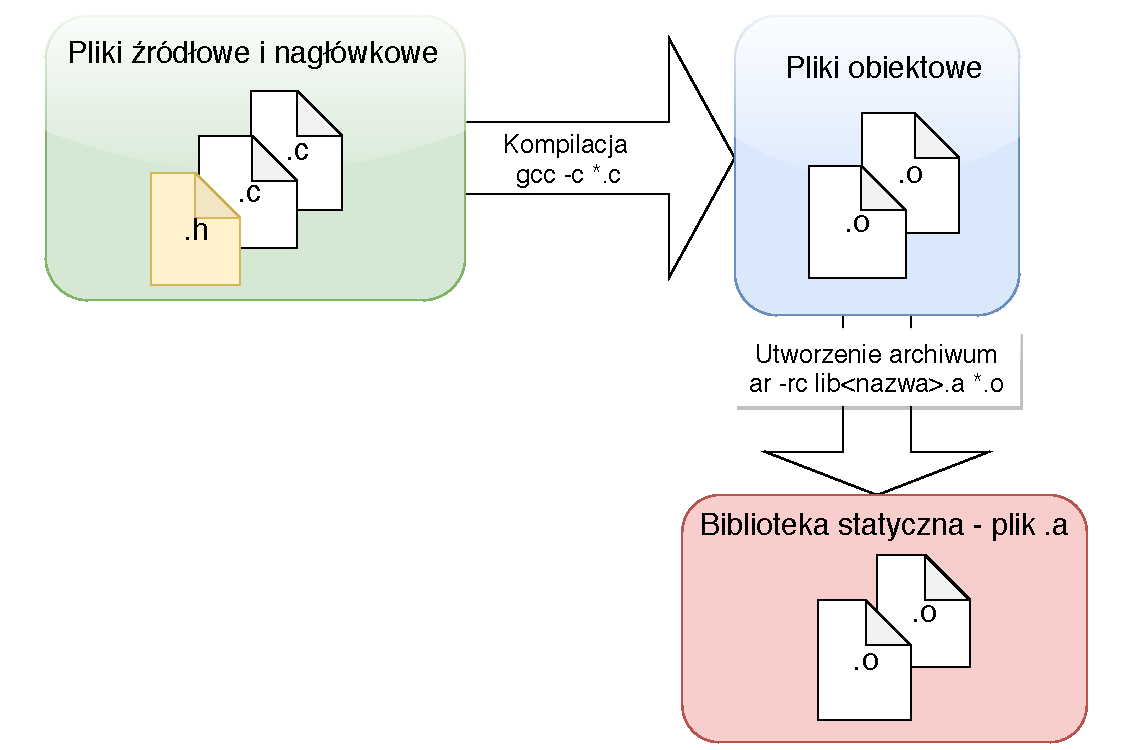
\includegraphics[width=\textwidth]{images/StaticLibFlow}
\end{figure}

Zawartość powstałego archiwum można zbadać za pomocą komendy \textit{ar -t} - wyświetla ona wszyskie pliki obiektowe wchodzące w skład danej biblioteki. Istnieje również możliwość wylistowania symboli - służy do tego narzędzie \textit{nm}. Użycie tych narzędzi na wykonanym przez autorów przykładzie ilustruje listing \ref{lst:libstat3}. Wynikiem polecenia \textit{nm} są tam dwa symbole, oznaczające dwie udostępnione dla użytkowników biblioteki funkcje (dodawanie i odejmowanie liczb zespolonych).

\begin{lstlisting}[language=bash, caption={Użycie poleceń \textit{ar -t} oraz \textit{nm} na bibliotece statycznej.},label={lst:libstat3}]
user@host:~/complex$ ar -t libcoml.a
complex_opers.o
user@host:~/complex$ nm libcoml.a

complex_opers.o:
0000000000000000 T add_complex_numbers
0000000000000091 T subtract_complex_numbers
\end{lstlisting}


\paragraph*{Dołączanie utworzonej biblioteki do programu}\mbox{}\\
Rysunek \ref{fig:staticliblink} przedstawia schematycznie proces dołączania utworzonej biblioteki statycznej do programu. Proces ten składa się z następujących etapów:

\begin{figure}[H]
\centering
\caption{Proces dołączania biblioteki statycznej do programu z uwzględnieniem komend koniecznych do wykonania poszczególnych etapów}
\label{fig:staticliblink}
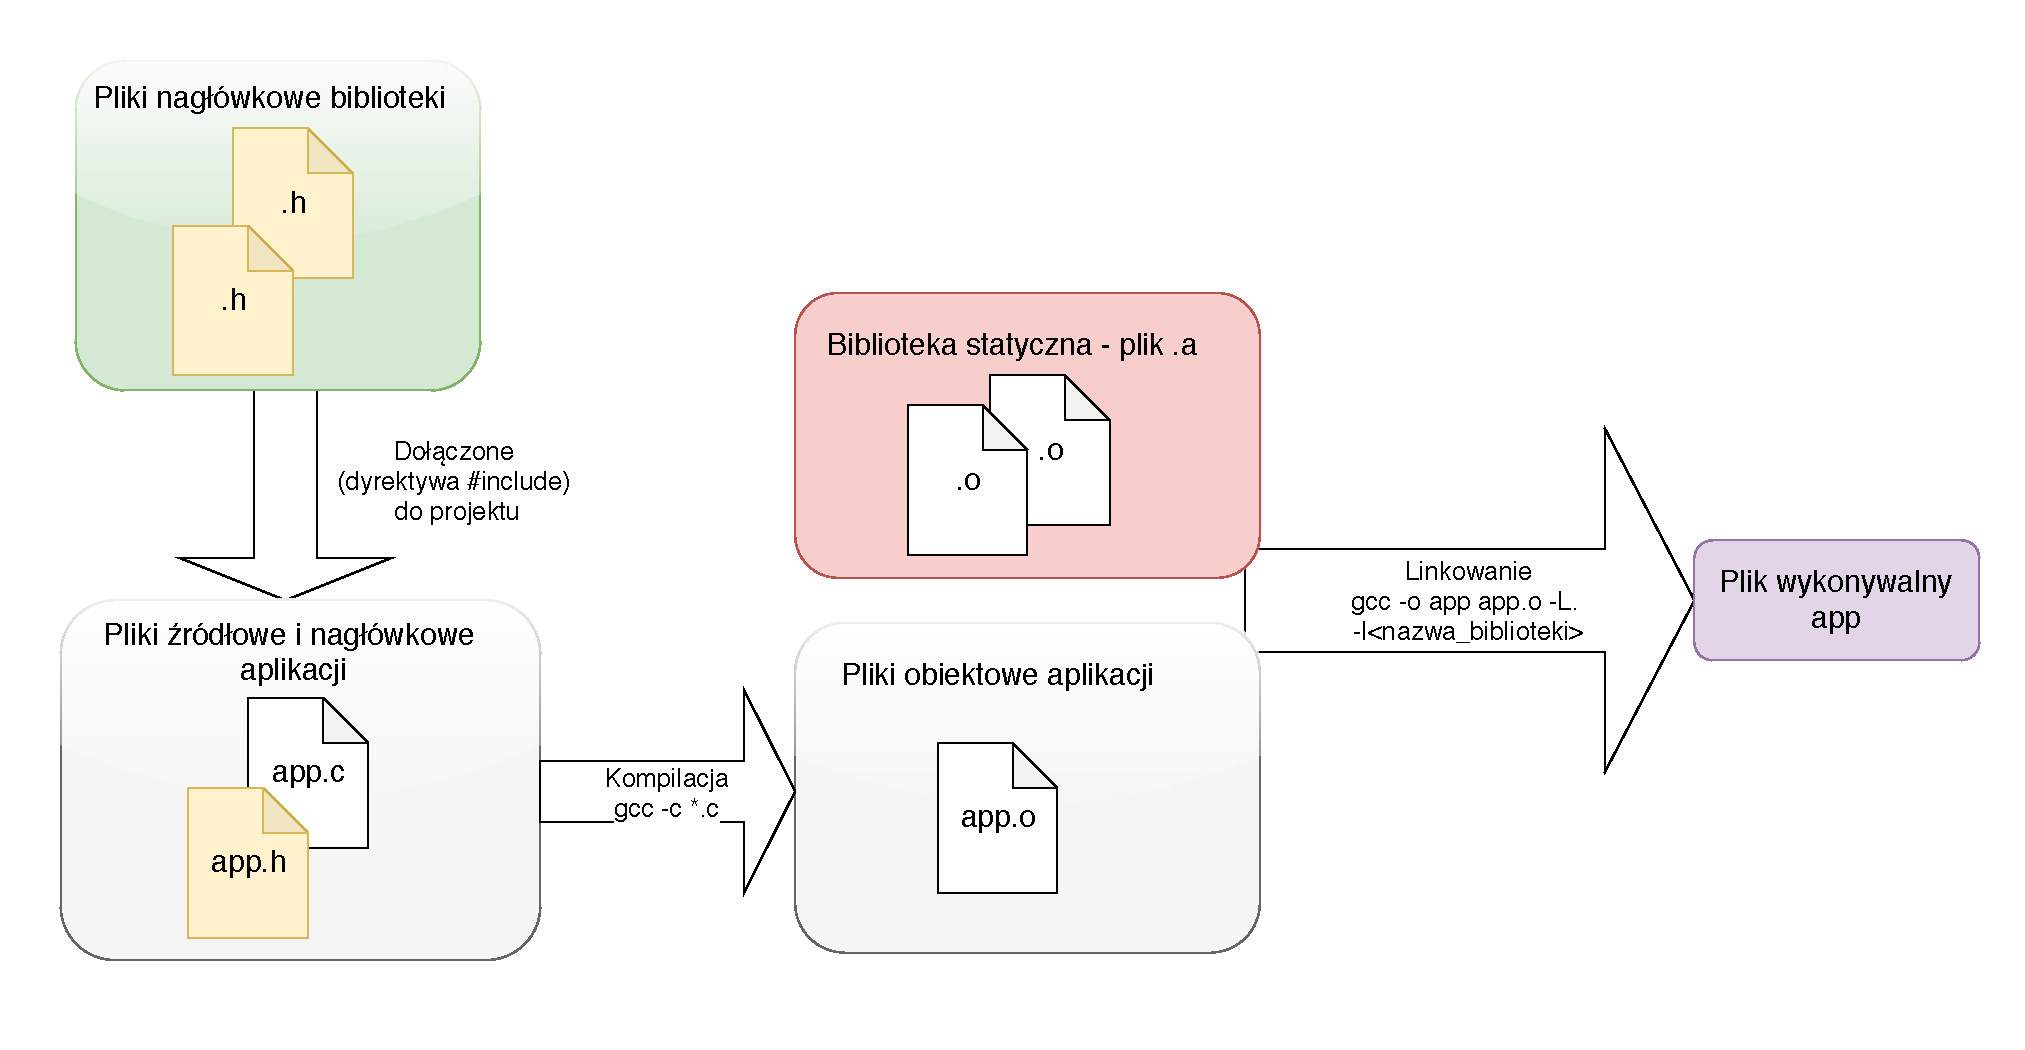
\includegraphics[width=\textwidth]{images/StaticLibLink}
\end{figure}

\begin{itemize}
\item dołączenie do źródeł programu plików nagłówkowych zawierających deklaracje stanowiące interfejs między programem a biblioteką (dyrektywa \textit{include} - listing \ref{lst:libstat4}).

\begin{lstlisting}[language=c++, caption={Plik \textit{app.c} zawierający dyrektywę \textit{include} dołączającą plik nagłówkowy zawierający deklaracje funkcji z biblioteki statycznej},label={lst:libstat4}]
#include "../complex/complex_opers.h"
#include <stdio.h>

int main(void) {

    complex_number a = {2.5, 3.7};
    complex_number b = {3.5, 0};

    complex_number c = add_complex_numbers(a, b);
    complex_number d = subtract_complex_numbers(a, b);

    printf("%lf %lf\n", c.real, c.imaginary);
    printf("%lf %lf\n", d.real, d.imaginary);

    return 0;
}
\end{lstlisting}

\item kompilacja plików źródlowych programu do postaci plików obiektowych za pomoca \textit{gcc} (listing \ref{lst:libstat5}). Wynikiem powinien być zestaw plików obiektowych odpowiadający wykorzystanym plikom źródłowym.

\begin{lstlisting}[language=bash, caption={Kompilacja plików źródłowych głównego programu do postaci obiektowej.},label={lst:libstat5}]
user@host:~/app$ gcc -c *.c
user@host:~/app$ ls
app.c  app.o
\end{lstlisting}


\item połączenie plików obiektowych i biblioteki w plik wykonywalny za pomocą \textit{gcc} (listing \ref{lst:libstat6}). Opcja \textit{-L} pozwala określić ścieżkę do dołączanej biblioteki, natomiast \textit{-l} - nazwę bibliteki (bez przedrostka \textit{lib} i rozszerzenie \textit{.a}).

\begin{lstlisting}[language=bash, caption={Linkowanie plików obiektowych programu z biblioteką statyczną, wynik uruchomienia programu obrazuący poprawne działanie przykładu.},label={lst:libstat6}]
user@host:~/app$ gcc -o app app.o -L../complex -lcoml
user@host:~/app$ ls
app  app.c  app.o
user@host:~/app$ ./app
6.000000 3.700000
-1.000000 3.700000
\end{lstlisting}

\end{itemize}

\subsection{Biblioteki współdzielone}



\paragraph*{Tworzenie biblioteki współdzielonej}\mbox{}\\
\paragraph*{Dołączanie utworzonej biblioteki do programu}\mbox{}\\
\paragraph*{Wersjonowanie bibliotek współdzielonych}

\subsection{Porównanie rodzajów bibliotek}


\section{Narzędzie CMake}

\textit{CMake (Cross-platform Make)} to narzędzie pozwalające na konfigurację procesu budowania oprogramowania (aplikacji oraz bibliotek) w sposób niezależny od platformy. Jego działanie opiera się na generowaniu pliku budującego natywnego dla określonej platformy \cite{CMakeIntro} (dla systemów z rodziny UNIX jest nim \textit{Makefile}) na podstawie przygotowanego przez użytkownika pliku \textit{CMakeLists.txt}. Takie podejście w znacznym stopniu ułatwia tworzenie aplikacji multiplatformowych oraz pozwala na intuicyjne zarządzanie zależnościami w projekcie. Domyślnie CMake pracuje z językami C i C++, natomiast nowe wersje narzędzia wpierają ponadto m.in. język C\# czy technologię CUDA \cite{CMakeSupport}. Narzędzie to jest rozwijane i wspierane przez firmę \textit{Kitware}.\par

\paragraph*{Plik CMakeLists.txt}\mbox{} \\
Jak wspomniano wyżej działanie narzędzia CMake opiera się na przygotowanym przez użytkownika pliku (lub zestawie plików rozmieszczonych w strukturze katalogów projektu) \textit{CMakeLists.txt}. Plik ten zawiera polecenia napisane w specjalnie do tego celu przygotowanym języku skryptowym. Użytkownik może za jego pomocą  m.in. określać jakie pliki wykonywalne mają zostać wygenerowane podczas procesu budowania, wskazać lokalizację plików źródłowych czy określić zależności między komponentami projektu oraz bibliotekami zewnętrznymi. \par

\paragraph*{Prosty przykład}\mbox{} \\
Listing \ref{lst:hello} zawiera przykład prostego pliku \textit{CMakeLists.txt}, pozwalającego na zbudowanie napisanej w języku C++ obiektowej wersji klasycznego programu \textit{Hello world}. Przykład ilustruje zastosowanie podstawowych poleceń CMake do określenia minimalnej wersji narzędzia, standardu języka C++, wynikowego pliku wykonywalnego oraz potrzebnych plików nagłówkowych. \par

\begin{lstlisting}[language=bash,caption={Przykład prostego pliku CMakeLists.txt przeznaczonego do budowania programu napisanego w C++}, label={lst:hello}]
# Określenie minimalnej wersji CMake
cmake_minimum_required(VERSION 3.0 FATAL_ERROR)

# Określenie standardu języka C++
set(CMAKE_CXX_STANDARD 14)
set(CMAKE_CXX_STANDARD_REQUIRED True)

# Nazwa oraz wersja projektu
project(Hello VERSION 1.0)

# Dodanie pliku wykonywalnego, który powinien powstać
# wskutek procesu budowania
add_executable(Hello Main.cpp)

# Dodanie do projektu katalogu include wraz ze znajdującym się 
# wewnątrz niego plikiem nagłówkowym
target_include_directories(Hello PUBLIC "${CMAKE_CURRENT_SOURCE_DIR}/include")
\end{lstlisting}

\paragraph*{Wersje CMake}\mbox{} \\
CMake jest narzedziem, który w ciągu ostatnich kilku lat przechodzi gruntowne zmiany. Starsze wersje (np. 2.8) oparte są o prosty system zmiennych \cite{CMakeRight}, co wprowadza szereg trudności w zarządzaniu dużymi projektami z wielopoziomowymi drzewami zależności. Dodatkowym problemem tych wersji jest również brak dobrze zdefiniowanych tzw. \textit{dobrych praktyk} oraz nieprzystępna dla początkujących dokumentacja. Współczesne wersje narzędzie CMake (zwykle za takie uznaje się nowsze od wersji 3.0) opierają się na innym, bardziej ustrukturyzowanym \cite{CMakeRight} podejściu, co było przyczyną pojawienia się dla nich wyżej wspomnianych \textit{dobrych praktyk}. Zalecane jest więc, by nowe projekty prowadzone były właśnie z użyciem nowszych wersji narzędzia.

\paragraph*{Narzędzia CTest i CPack}\mbox{} \\
CMake oferuje również możliwość konfiguracji sposobu testowania projektu. Służy do tego narzędzie \textit{CTest}, dystrybuowane razem z podstawowym narzędziem CMake. Innym przydatnym modułem jest \textit{CPack} - narzędzie to służy przygotowywaniu pakietów instalacyjnych z oprogramowaniem. Użycie obu wymienionych narzędzi polega na umieszczeniu w pliku \textit{CMakeLists.txt} kilku przeznaczonych do tego komend. \par 


\section{Język Python}
\textit{Python} jest nowoczesnym, wysokopoziomowym językiem programowania, wspierającym takie paradygmaty jak programowanie obiektowe czy imperatywne. Działanie Pythona opiera się na dynamicznym systemie typów. Z założenia Python jest językiem przyjemnym w użytkowaniu, co przyczyniło się do jego dużej popularności \cite{Lutz}. Python jest szeroko stosowany jako język skryptowy - takie też zastosowanie znalazł w projekcie GGSS.

\paragraph*{Prosty przykład}\mbox{} \\
Listing \ref{lst:pyexample} przedstawia prosty przykład skryptu napisanego w języku Python w wersji 3. Kod ten stanowi uproszczoną wersję skryptu zaprezentowanego w dalszej części pracy, którego zadaniem jest zbudowanie aplikacji w zależności od przekazanych przez użytkownika argumentów. Przykład prezentuje prosty skrypt przyjmujący jeden z dwóch możliwych argumentów i wypisujący informację na temat otrzymanego argumentu na standardowe wyjście.

\begin{lstlisting}[language=python,caption={Przykład prostego skryptu napisanego w języku Python 3 - przetwarzanie argumentów podanych przez użytkownika do skryptu}, label={lst:pyexample}]
import argparse

## Prosty skrypt przetwarzający argumenty podane 
## przy jego uruchomieniu przez użytkownika

## Definicja funkcji w języku Python
def parse_command_line_arguments():

    ## Obiekt przetwarzający argumenty (parser)
    parser = argparse.ArgumentParser()

    ## Argumenty wzajemnie się wykluczające
    group = parser.add_mutually_exclusive_group(required=True)
    group.add_argument("-s", "--staticboost", 
        help="Use static Boost linking.", action="store_true")
    group.add_argument("-d", "--dynamicboost",
        help="Use dynamic Boost linking.", action="store_true")

    return parser.parse_args()

if __name__=="__main__":
    ## Wywołanie funkcji
    arguments = parse_command_line_arguments()
    print(arguments)


\end{lstlisting}

\paragraph*{Wersje języka Python}\mbox{} \\
Python funkcjonuje w dwóch wersjach: Python 2 oraz 3. Wersje te nie są ze sobą w pełni kompatybilne, tzn. pewne funkcjonalności Pythona 2 nie są dostępne w Pythonie 3 i odwrotnie. Różnice znaleźć można również np. w domyślnym sposobie kodowania łańcuchów znakowych (ASCII w Pythonie 2, Unicode 2 Pythonie 3) oraz w wyniku dzielenia (za pomocą operatora \textit{/}) dwóch liczb całkowitych (w Pythonie 2 wynikiem jest liczba całkowita, w Pythonie 3 liczba zmiennoprzecinkowa typu \textit{float}) \cite{Python2vs3}. Ponadto zakończenie oficjalnego wsparcia Pythona w wersji 2 przewidziane jest na styczeń 2020 roku \cite{Python2Countdown} - co w momencie pisania niniejszej pracy (grudzień 2019) jest terminem niedalekim i miało kluczowe znaczenie w czasie podejmowania pewnych decyzji projektowych.

\paragraph*{Zewnętrzne biblioteki}\mbox{} \\
Jedną z największych zalet Pythona jest bardzo duża liczba bibliotek zewnętrznych tworzonych przez społeczność Pythona. Rozbudowują one język o wiele nowych funkcjonalności, np. przetwarzanie plików HTML czy wykonywanie obliczeń numerycznych. W niniejszej pracy zastosowanych zostało kilka tego typu bibliotek, m.in. \textit{Beautiful Soup} do wspomnianego wyżej przetwarzania dokumentów w formacie HTML. Omówienie ich działania na przykładach znaleźć można w dalszej części pracy - przy opisie konkretnego ich zastosowania. 



\section{Język powłoki bash}
\section{System kontroli wersji Git i portal Gitlab}
\section{Manager pakietów - RPM}
\section{Technologie wirtualizacji i konteneryzacji}
